\documentclass[11pt]{article}
\usepackage{amsmath, amssymb, amsthm}
\usepackage[retainorgcmds]{IEEEtrantools}

\usepackage[pdftex]{graphicx}

\usepackage{fancyhdr}

%Format stuff
\pagestyle{fancy}
\headheight 35pt

%Header info
\chead{\Large \textbf{Integrals and Derivatives on Curves}}
\lhead{}
\rhead{}

\begin{document}
\section{Line Integrals}
	Picture a function $\mathbb{R}^3 \xrightarrow{\vec{F}} \mathbb{R}^3$ defined in a region $D$ as a \textbf{vector field}, an assignment of the vector $\vec{F}(\vec{x})$ to each point in $D$. If there is a curve $\gamma$ in $D$ parametrized by $g(t)$ continuously differentiable for $a \leq t \leq b$, then the \textbf{line integral} of $\vec{F}$ over $\gamma$ is
	\begin{equation}
		\int_a^b \vec{F}(g(t)) \cdot g'(t)dt
	\end{equation}
	
	The \textbf{circulation} of $\vec{F}$ over $\gamma$ is defined as the value of the integral of $\vec{F}$ over a curve $\gamma$. 
	
	\subparagraph{Work} Work is the amount of force applied in the direction of movement. Given $\vec{F}$ describes a force field and $\gamma$ is a continuously differentiable curve, 
	\begin{equation}
		W = \int_a^b \vec{F}(g(t)) \cdot g'(t)dt = \int_\gamma \vec{F} \cdot \vec{t} ds
	\end{equation}
	where $ds = |g'(t)|dt$ is called the \textbf{arc-length differential}.
	
	\subparagraph{Equivalent Parametrizations} When different parametrizations describe the same image curve, they are equivalent if each segment of the image curve is traced the same number of times and tangent vectors point in the same direction. In general, the parametrizations
	\begin{equation}
		\vec{x} = f(t), \quad a \leq t \leq b \quad \text{and} \quad \vec{x} = g(u), \quad \alpha \leq u \leq \beta
	\end{equation}
	are equivalent if there is a continuously differentiable function $\phi$ with $\phi ' > 0$ from $[\alpha, \beta]$ onto $[a, b]$ such that $f(\phi(u)) = g(u)$. Equivalent parametrizations of a curve $\gamma$ yield the same value for 
	\begin{equation*}
		\int_\gamma \vec{F} \cdot d\vec{x}
	\end{equation*}
	

	\subparagraph{Fundamental Theorem of Calculus} If $f$ is a continuously differentiable real-valued function and $\gamma$ is smooth in $D$,
		\begin{equation}
			\int_\gamma \nabla f \cdot d\vec{x} = \int_{\vec{a}}^{\vec{b}} \nabla f \cdot d\vec{x} = f(\vec{b}) - f(\vec{a})
		\end{equation}
		More generally, the solution to $\nabla f(\vec{x}) = \vec{F}(\vec{x})$ with $f(\vec{x_0}) = 0$ is
		\begin{equation}
			f(\vec{x}) = \int_{\vec{x}_0}^{\vec{x}_1} \vec{F}(\vec{x}) \cdot d\vec{x}
		\end{equation}
		
\section{Weighted Curves and Surfaces of Revolution}
	The arc length of a curve parametrized by $\vec{x} = g(t)$ is defined by
	\begin{equation}
		s(t) = \int_{t_0}^t |\vec{x}'(u)| du
	\end{equation}
	Because a path can be traced at any speed, it is useful to parametrize a curve by arc length. If the points in the image are one-to-one with arc length from an origin point on the curve, then it is \textbf{parametrized by arc length} if $|g'(t)| = 1$. In this case, the expression $|\vec{x}'(t)|dt = |g'(t)|dt$ is called the \textbf{arc length element}.
	
	\subparagraph{Weighted Curves} Imaging a weight function $\mu$ that assigns a weight $\mu(h(s))$ to each point $h(s)$ at distance $s$ along a curve parametrized by its arc length. Then the total mass of the curve is
	\begin{equation}
		M = \int_{s_0}^{s_1} \mu(h(s))ds
	\end{equation}
	If the curve is not parametrized by arc length, the arc length function $s$ is
	\begin{equation}
		s(t) = \int_{t_0}^t |g'(u)|du
	\end{equation}
	and after changing variables,
	\begin{equation}
		M = \int_{s_0}^{s_1} \mu(h(s))ds = \int_{t_0}^{t_1} \mu(h(s(t)))\frac{ds(t)}{dt}dt = \int_{t_0}^{t_1} \mu(g(t))|g'(t)|dt
	\end{equation}
	
	\subparagraph{Surfaces of Revolution} A surface of revolution is generated by rotating a plane curve about a fixed line in the same plane. The surface area of the surface of rotation $S$ with respect to arc length is
	\begin{equation}
		\sigma (S) = \int_{s_1}^{s_2} 2\pi r(s)ds
	\end{equation}
	In a 2D application rotating a curve with $y(t) \geq 0$, after substituting for the appropriate arc length element with respect to $t$,
	\begin{equation}
		\sigma (S) = \int_{t_0}^{t_1} 2\pi y(t) \sqrt{x'(t)^2 + y'(t)^2} dt
	\end{equation}
	
\section{Normal Vectors and Curvature}
	Given a twice continuously differentiable curve $\vec{x}(t)$,
	\begin{equation}
		\frac{ds}{dt}(t) = s'(t) = |\vec{x}'(t)|
	\end{equation}
	The vector of length 1 in the direction of the velocity vector is usually denoted $\vec{t}(t)$.  Thus, $\vec{x}'(t) = s'(t)\vec{t}(t)$ or $\vec{t} = \vec{x}' / s'$.
	
	The acceleration vector along the curve is
	\begin{equation}
		\vec{x}'' = s''\vec{t} + s'\vec{t}'
	\end{equation}
	The vector $\vec{t}'(t)$ is orthogonal to $\vec{t}(t)$, and when $\vec{t}'(t) \neq 0$, we define a unit vector $\vec{n}(t)$ called the \textbf{principal normal} such that $\vec{t}' = |\vec{t}'|\vec{n}$. Thus, the acceleration vector can also be expressed as
	\begin{equation}
		\vec{x}'' = s''\vec{t} + s'|\vec{t}'|\vec{n}
	\end{equation}
	
	As figure \ref{fig:normal} shows, the two orthogonal components $\vec{a}_t = s''\vec{t}$ and $\vec{a}_n = s'|\vec{t}'|\vec{n}$ are called the \textbf{tangential acceleration} and \textbf{centripetal acceleration} respectively.
	
	\begin{figure}[htb]
		\centering
		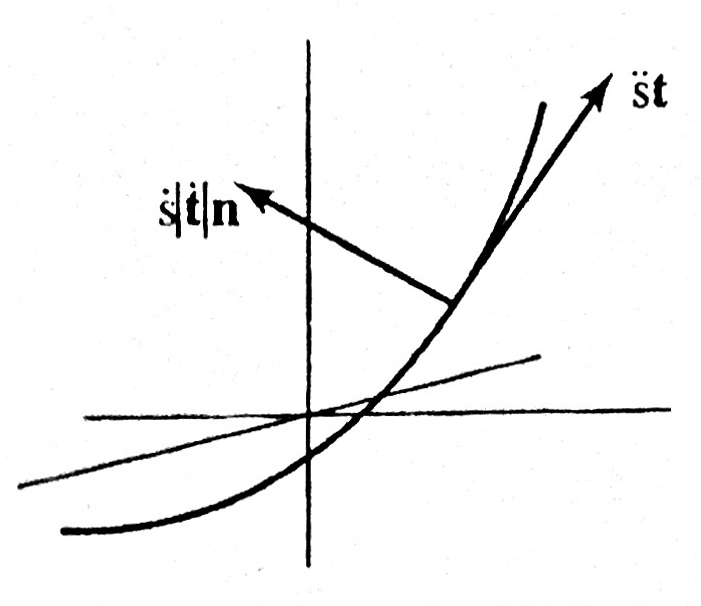
\includegraphics[width=0.3\textwidth]{normal.png}
		\caption{Acceleration vectors}
		\label{fig:normal}
	\end{figure}
	
	The \textbf{curvature} at $\vec{x}(t)$ is the scalar
	\begin{equation}
		\kappa(t) = \left| \frac{d\vec{t}}{ds} \right|
	\end{equation}
	and measures the turning rate of the unit tangent $\vec{t}$, viewed as a function of arc length. For a twice-differentiable smooth curve $\vec{x}(t)$, the curvature function is
	\begin{equation}
		\kappa = \frac{|\vec{t}'|}{s'}
	\end{equation}
	and therefore the acceleration vector is
	\begin{equation}
		\vec{x}'' = s''\vec{t} + (s')^2\kappa \vec{n}
	\end{equation}
	Another two equations for computing curvature, the first in terms of $\vec{x}'$ and $\vec{x}''$ and the second for $y = f(x)$.
	\begin{equation}
		\kappa(t) = \frac{\sqrt{|\vec{x}'|^2 |\vec{x}''|^2 - (\vec{x}' \cdot \vec{x}'')^2}}{|\vec{x}'|^3}
	\end{equation}
	\begin{equation}
		\kappa(x) = \frac{y''}{(1 + (y')^2)^{3/2}}
	\end{equation}
	
\section{Flow Lines, Divergence, and Curl}
	\subparagraph{Flow Lines} A differentiable curve $\vec{x} = \vec{x}(t)$ is called a flow line of the vector field $\vec{F}(x)$ if $\vec{x}'(t) = \vec{F}(\vec{x}(t))$ in some interval and represents the path a particle takes in a fluid. If $\vec{F}$ is a gradient field such that $\vec{x}' = \vec{F} = \nabla f(\vec{x})$, then the flow lines are perpendicular to the level sets of $f$.
	
	\subparagraph{Divergence} Divergence of a vector field div$\vec{F}(x)$ is the sum of the main diagonal elements of the matrix $\vec{F}'$ and represents the expansion rate of fluid per unit of area and volume. div can also be expressed as
	\begin{equation}
		\text{div} \vec{F} = \nabla \cdot \vec{F}
	\end{equation}
	Given a density equation $\rho (\vec{x})$, div can be expressed as the \textbf{continuity equation}
	\begin{equation}
		\text{div} \vec{F}(\vec{x}) = -\frac{\partial \rho}{\partial t} (\vec{x})
	\end{equation}
	
	\subsection{Curl} 
		In 3 dimensions, the curl of a differentiable vector field $\vec{F} = F_1 \vec{i} + F_2 \vec{j} + F_3 \vec{k}$ is
		\begin{equation}
			\text{curl}\vec{F} = \left(\frac{\partial F_3}{\partial y} - \frac{\partial F_2}{\partial z} \right) \vec{i} + \left(\frac{\partial F_1}{\partial z} - \frac{\partial F_3}{\partial x} \right) \vec{j} + \left(\frac{\partial F_2}{\partial x} - \frac{\partial F_1}{\partial y} \right) \vec{k}
		\end{equation}
		or, more easily,
		\begin{equation}
			\text{curl}\vec{F} = \nabla \times \vec{F}
		\end{equation}
		
		\subparagraph{Scalar curl} The curl of a 2-dimensional vector field, taken as a slice of a 3-dimensional field where $\vec{k}$ is identically 0 and $F_1$ and $F_2$ are independent of $z$ is
		\begin{equation}
			\text{curl} \vec{F}(x, y) = \left(\frac{\partial F_2}{\partial x} - \frac{\partial F_1}{\partial y} \right)\vec{k}
		\end{equation}
		The \textbf{scalar curl} of this field is the coefficient of the basis vector, and measures the local tendency of a vector field to form a vortex.
		
		\subparagraph{Interpretation of Curl} Let $P$ be a plane through $\vec{x}$. For each point of $P$ that is also in the domain of $F$, project $\vec{F}(\vec{x})$ perpendicularly onto $P$ to get a 2-dimensional vector field $\vec{F}_n$ in $P$.
		\begin{itemize}
			\item $|\text{curl} \vec{F}(\vec{x})|^2 = |\text{curl}\vec{F}_n(\vec{x})|^2 + (\vec{n} \cdot \text{curl}\vec{F}(\vec{x}))^2$
			\item Choosing $\vec{n}$ perpendicular to curl$\vec{F}(\vec{x})$, meaning the vector curl$\vec{F}(\vec{x}))$ is parallel to $P$, maximizes the absolute value of the scalar curl.
			\item If curl$\vec{F}_n(\vec{x}) > 0$ in a neighborhood of a point, then the circulation of $\vec{F}_n$ around nearby circular paths centered at the same point in $P$ is positive following the right hand rule.
		\end{itemize}
%	\begin{center}
%	\begin{tikzpicture}
%		[scale=3,line cap=round,
%		%Styles
%		axes/.style=,
%		important line/.style={very thick},
%		information text/.style={rounded corners,fill=red!10,inner sep=1ex},
%		dot/.style={circle,inner sep=1pt,fill,label={#1},name=#1}			
%		]
%		
%		%Colors
%		\colorlet{anglecolor}{green!50!black}	%angle arcs/lines
%		
%		%The graphic
%	\end{tikzpicture}
%	\end{center}

%	\begin{figure}[htb]
%		\centering
%		\includegraphics[width=0.8\textwidth]{filename.eps}
%		\caption{Caption.}
%		\label{fig:figure}
%	\end{figure}

%		\def\enotesize{\normalsize}
%		\theendnotes
\end{document}